\section{Evaluation}\label{sec:evaluation}
We evaluate scheduling overhead and scheduling performance.
Scheduling experiments are limited on the GPU scheduling since CPU scheduling performance is already experiments~\cite{kato:resch}.
In this evaluation, we focus two point.
The one is to indicate the Linux-RTXG disadvantages,
the other one is QoS performance comparing prior work. 

%本実験では2点にフォーカスし評価を行う.
%まず一つ目は,本Linux-RTXGを利用した際のオーバヘッドを定量的に計測し、利用に伴ってどれだけのデメリットを含んでいるかを提示する
%2つ目に,シンクロナイゼーション方式がカーネル編集を含まない方式でどの程度のパフォーマンス維持が可能であるかを示す.

GPU using Real-world oriented applications\cite{hirabayashi:cpsna2013,tokamak} are executed cyclic.
%今回の評価用アプリケーションは周期的に実行されるため,リアル・ワールドのアプリケーションと同等の処理フローであるとし評価で用いる.
This evaluation applications are equivalent to the real-world oriented applications
because GPU applications characteristics are these application on the single GPU kernel.
%GPUを利用するリアル・ワールドのアプリケーション\cite{hirabayashi,tokamak}ではGPUタスクの多くは周期的に実行される.
We will discuss in the next chapter for the difference between the functions and features to hold to it with a qualitative evaluation.
%定性的な評価としては関連する研究と保持する機能や特徴の差について次章でdiscussする。

\TODO{GPUSyncと比較しなくて良いのか}


\subsection{Experimental Environment}
Our experiments are conducted with the Linux kernel 3.16.0 on NVIDIA Geforce GTX680 graphics card and 3.40GHz Intel Core i7 2600, which contains 8 cores (including the two hyper-threading cores) and 8GB main memory.

GPU programs are written in CUDA and compiled by NVCC v6.0.1.
GPU drivers are used NVIDIA driver 331.62 and Nouveau driver linux-3.16.0.
CUDA libraries are used NVIDIA CUDA-6.0 and Gdev.
%CPUはIntel Core i7 2600 3.40GHz、
%4GB*2のメモリ、GPUはGeForce GTX680を用いる。
%KernelはLinux kernel 3.16.0を用い、ディストリビューションはUbuntu 14.04である。
%CUDAコンパイラはNVCC v6.0.1、CUDAランタイムはcuda-6.0 or Gdev、GPUドライバはNVIDIA (331.62)、Nouveau (linux-3.16.0)を用いる。
%各ランタイム、ドライバは評価項目ごとに使い分ける。

\subsection{Interrupt intercept overhead}
We mesurement overhead due to interrupt interception.
%Interrupt interceptのオーバヘッドの測定を行う。
This experiment use GPU driver which is used the Nouveau in order to compare and identify the type of interrupt.
We compare consumption time from the start ISR until ISR is completion, it consumption time is average time of 1000 times.

%本評価では、GPUドライバはnouveauを用いる。

%割り込み処理は、各割り込みの種類によって、処理時間が異なり、その分布は一様ではないため、単に測定して平均をとっても比較ができない。
%そのため各割り込みの種類の判別のためにNouveauを用いて、割り込みの種類が同一のもので、カーネル内のdo\_IRQ関数内でハンドラが呼ばれてから終了までの時間を測定し
%どの程度のオーバヘッドで割り込みの盗聴及び、盗聴した割り込みがいずれのカーネルに関連したものであるかの識別ができるかどうかを測定する。

\begin{figure}[t]
\begin{center}
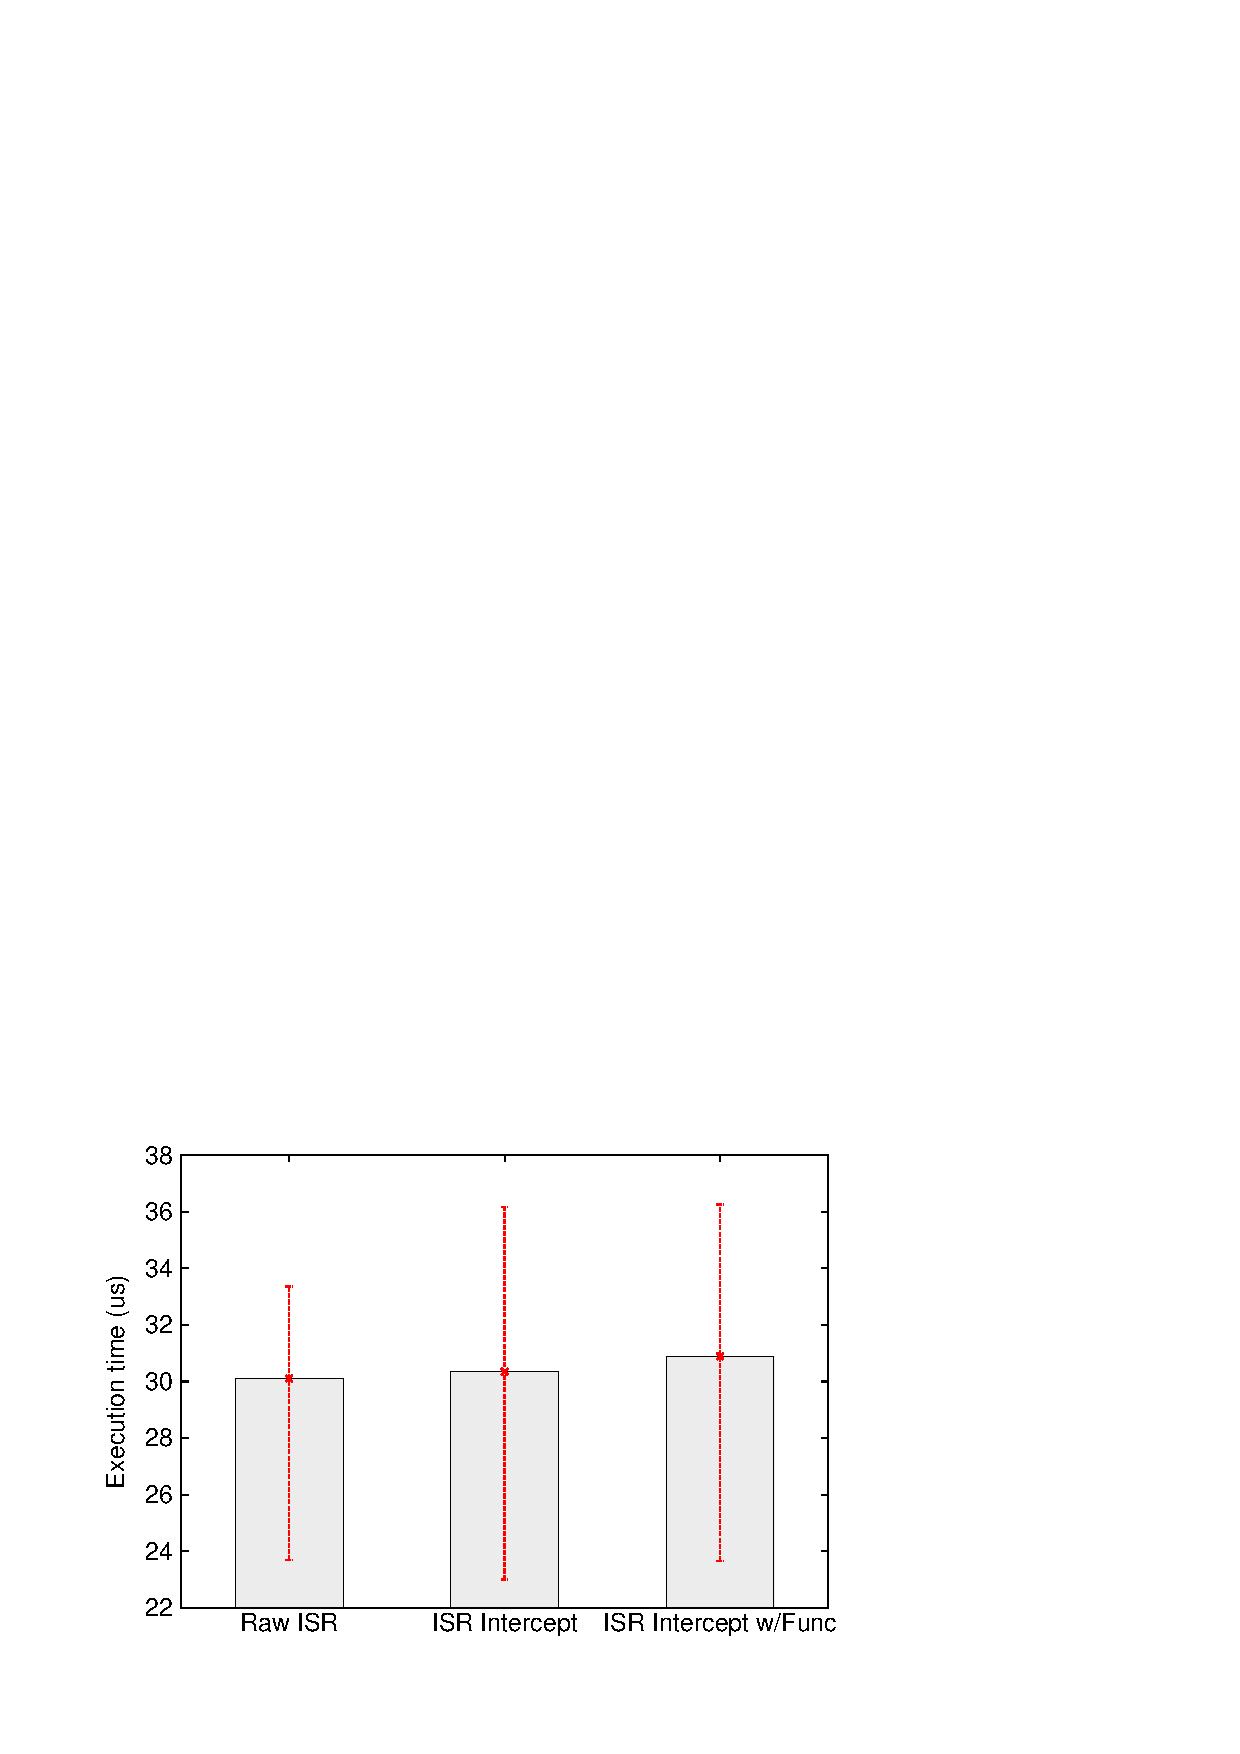
\includegraphics[width=0.4\textwidth]{img/interrupt.pdf}
\caption{Interrupt intercept overhead}
\end{center}
\label{fig:irq_overhead}
\end{figure}

Figure~\ref{irq_overhead} shows results of mesurements in the above setting.
%Figure \ref{irq_overhead}は上記設定で測定した結果である。
Raw ISR is execute ISR in the normal routine, ISR Intercept is only intercept our approach,
ISR intecept w/Func is interception and processing functions that are identify the ISR and wakeup the scheduler thread.
These are showed the average times with error bar is indicate minimum and maximum.

As a result, the overhead exist certainly.
ISR Intercept has overhead that is about 247 nano seconds.
ISR Intercept w/Func also has overhead that is about 790 nano seconds.

Intuitively, it value does not affect system since very small values,
however, interrupt is occured frequently including such as timer interrupt, should be aware as disadvantages.

In addition, we evaluate comparing the response time of the ISR (top-half) and the tasklet (bottom-half) in an environment with noCPU load,
it evaluate does measurement time until the responsible timing from the start of interrupt process which is $do\_IRQ$ function is called).
it mesasurement result is shown in Figure~\ref{fig:bottomvstasklet}.

\begin{figure}[t]
\begin{center}
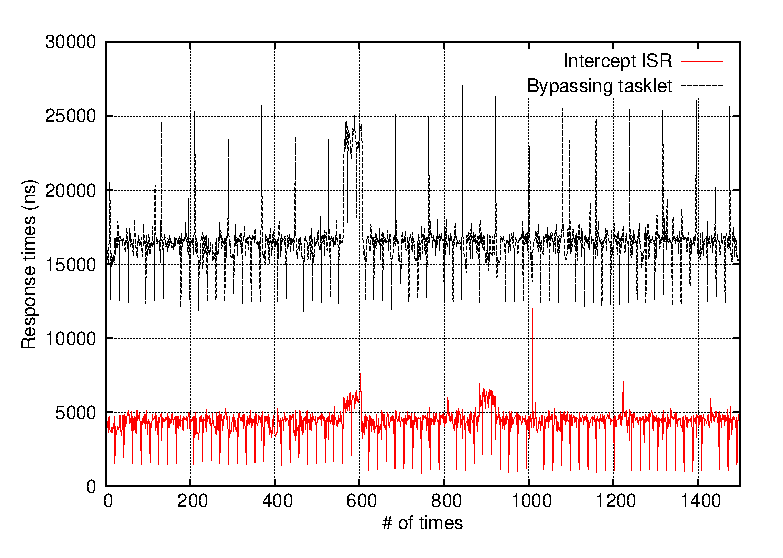
\includegraphics[width=0.4\textwidth]{img/tasklet_vs_interrupt}
\caption{Comparison of the response time of the interrupt top-half and bottom-half}
\end{center}
\label{fig:bottomvstasklet}
\end{figure}

GPUSync bypass the $tasklet\_schedule()$ if it function is called from the nvidia driver.
The tasklet is generally called after the important procesing in ISR.
It approach has robustness, but response is worse than ISR, it response can be seen from Figure~\ref{fig:bottomvstasklet}.


%Raw ISRは通常のルーチンで実行されるISR、ISR Interceptは割り込みを盗聴するのみ、
%ISR intercept w/Funcは盗聴した上でその割り込みが、いずれのカーネルに関連した割込みか識別しスケジューラを立ち上げる機能を実行した場合である。
%それぞれ1000回の測定で平均値を取り、最小値と最大値についてエラーバーで示している。
%この図から見て取れるように、オーバヘッドは確実に存在する。
%ISR Interceptだと247nsのオーバヘッドであり、
%ISR Intercept w/Funcでも790nsのオーバヘッドである。
%この数値は直感的に考えると小さくシステム自体に影響を及ぼすほどではないと考えられ、
%しかしその割込みが乱発することによる積み重ねによっては影響を与えることは、
%本手法のデメリットとして意識しなければならない。

\subsection{Independent Synchronization mechanism overhead}
We evaluate the overhead according to using independent synchronization mechanism.
The our method is need to call the $rtx\_nvrm\_notify()$ at the timing of requested synchronization (e.g. after the kernel launch issue). 
%本稿では同期生成のためのオーバヘッドを測定する。
%割込みの立ち上げは同期を求めるタイミング(e.g. カーネルラウンチ後)にrtx\_nvrm\_notify()を呼び出す必要がある。
In vanilla environment, these api is not necessary, therefore, time the API consumed is overhead.
%スケジューリングを行わないVanillaな状態ではこれらのAPIは必要ではないものであるため、これらのAPIにかかった時間はすべてオーバヘッドとなる。

We measured overhead by measuring the API consumed time between API call and return.
%そのためこれらのオーバヘッドの計測を行う。計測はAPIの呼び出しから戻るまでを測定する。

\begin{figure}[!t]
\begin{center}
\subfigure[Part of Initialize]{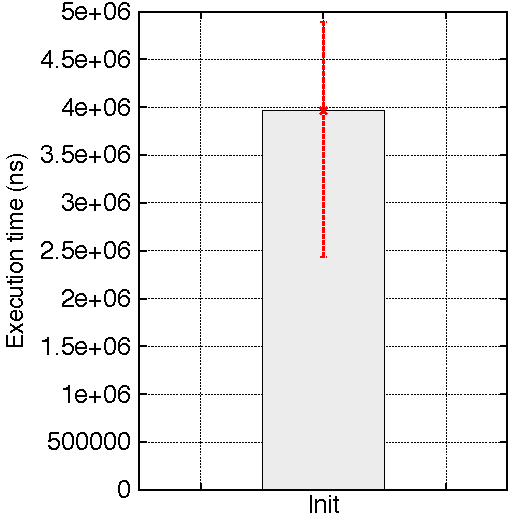
\includegraphics[width=0.23\textwidth]{img/irq_rise_init.pdf}}\subfigure[Part of notify]{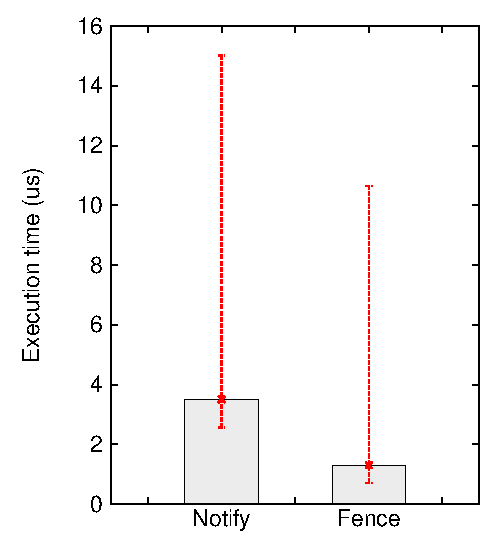
\includegraphics[width=0.23\textwidth]{img/irq_rise_notify.eps}}
\caption{Interrupt raised method overhead}
\label{fig:irq_rise_overhead}
\end{center}
\end{figure}

As a result shown in Figure~\ref{fig:irq_rise_overhead}.
Initialize is need to called the at awaken a linux process for allocating a indirect buffer and register several compute engine to the device driver.
Notify and Fence areGPU command sending to GPU devices which called at timing of the need to synchronization such as after the kernel launch issues.
These methods execution time is variants occurred affected by ioctl system call.
%結果をFigure \ref{fig:irq_rise_overhead}に示す。
%InitializeはIndirect Bufferはプロセスが立ち上がるたびに、
%コマンド送信用のIndirect Bufferの確保や各エンジンの登録のために呼び出される必要がある。
%Notifyはカーネル実行後や非同期メモリコピー実行後のような同期を発生させたいタイミングで呼び出される。
%これらはioctlシステムコールによってユーザ空間とカーネル空間をまたいでる影響か、実行時間のバラ付きが大きく出ている。

Initialize average time is about 4 mill seconds, however, application is not affected too much because above characteristics is only called once.
%Initializeは比較的時間がかかっているが、1プロセスにつき一度しか呼ばれないため、アプリケーション全体への影響は少ないと考えられる。
Notify is not takes much time that is about 3.5µs.
Fence likewise be not takes much time that is about 2µs.
Although may be not have to worry about for most applications,
it is necessary to consider the overhead in a cycle of short application.

\subsection{Scheduling Overhead}\label{sec:eval:sched_overhead}

\begin{figure}[t]
\begin{center}
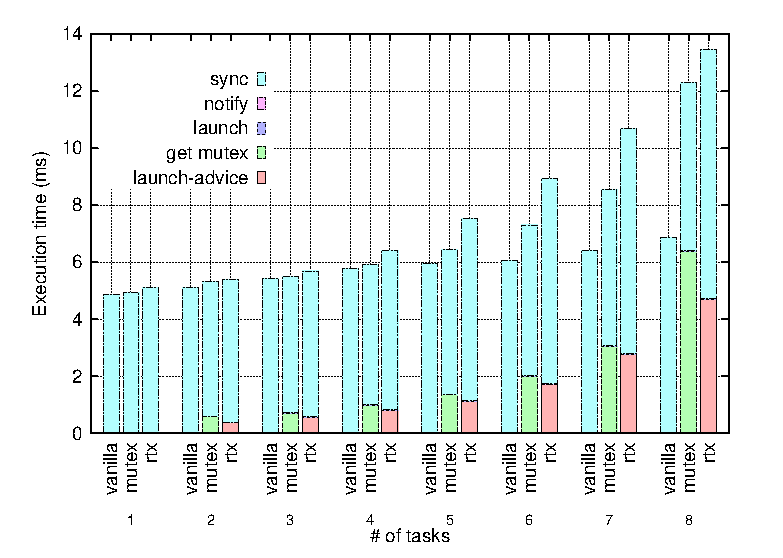
\includegraphics[width=0.5\textwidth]{img/sum_task_fp.eps}
\caption{Scheduling overhead(between GPU kernel launch request and synchronization)}
\end{center}
\label{fig:fp_overhead}
\end{figure}

\begin{figure}[t]
\begin{center}
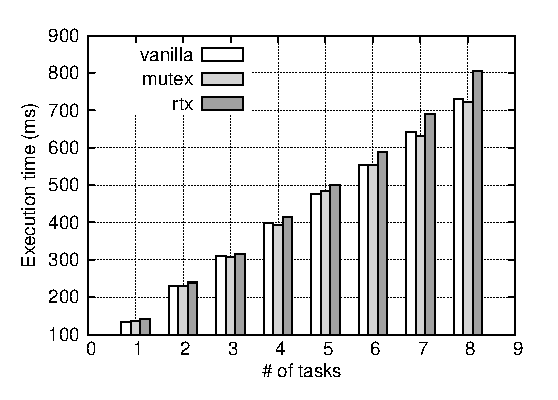
\includegraphics[width=0.5\textwidth]{img/sum_task.eps}
\caption{Scheduling overhead (Time of entire task)}
\end{center}
\label{fig:fp_overhead}
\end{figure}

We will evaluate scheduling overhead by using Linux-RTXG scheduler.
We prepared three applications that are "vanilla", "mutex", and "rtx" for mesurement overheads.
These applications is based common application based on Gdev's microbenchmark which has GPU looping function.
Changes are arranged to generate multiple GPU tasks by the fork.
Each tasks have 10 jobs, a job is included GPU data transferring and a GPU kernel execution.

The "rtx" application is scheduled by rtx.
The "mutex" application  is limited to single kernel issue similar to scheduling environment.
The "vanilla" application is not to change the base application.

CPU scheduing policies is using the simple fixed-priority scheduling by Linux-RTXG similar to Linux's \textbf{SCHED\_FIFO} that difference is the presence or absence of the job management.
GPU scheduling policies is fixed-priority scheduling with resrouce reservation witch is BAND scheduling policy.
The synchronization is using NOTIFY of independent synchronization mechanism.

We measured the average time in each part of each job of, 100 times GPU task execution (1000 jobs).
As a result show in Figure~\ref{fig:fp_overhead}.
%計測結果をFigure~\ref{fig:fp_overhead}に示す。
%アプリケーションに含まれるタスク数ごとにプロットしており、各ジョブ内のラウンチ要求から実行完了までにかかった時間の平均値を各処理毎に積み上げ式で示している。
The "launch\_advice" is time of until GPU kernel launch request is accept on the Linux-RTXG.
The "mutex" is time to get the mutex lock.
The "sync" is time of untile synchronizationed from issued the GPU kernel launch issue.



%launch\_adviceはrtx\_gpu\_launchによってGPU利用のためのリクエストを出してから、許可がでるまでを示しており、
%get\_mutexはmutexによってロックを獲得するまでの時間、
%launch、notifyはそれぞれコマンドを発行するまでにかかった時間で、
%syncは発行されてから同期完了するまでの時間である。
%全て、100回のアプリケーション実行($number of tasks ☓$)の平均値である.

%rtxでスケジューリングした場合のオーバヘッドを測定するために、"vanilla", "mutex", "rtx"の3種類のアプリケーションを用意した。
%全てに共通するのが、1個のアプリケーションに複数のタスクが存在しており、
%各タスクには10個のジョブが含まれることである。1個のジョブはGPUへのデータ転送、GPUカーネル実行、GPUからのデータ転送を含んでいる。GPUカーネルは単純な行列の計算を行う。
%
%3種で異なる点として、まずmutexは同時にlaunchが発行されるのが1つに調停されるようにmutexを用いてロックしたバージョンである。
%そしてrtxはlinxu-rtxgを用いて実行したケースであり、
%vanillaはそれらの追加が無くスケジューリングや調停を一切行わないケースである。


%CPUのスケジューリングはlinux-rtxを用いたシンプルなFixed-priorityスケジューリング (LinuxのSCHED\_FIFOと同様のポリシー、ジョブ管理のみを行う)を用いる。
%GPU側のスケジューリングは、Gdevで提案されたBANDスケジューラ、Linux-RTXでの同期は全てNOTIFYを用いて行う。


\subsection{Performance of QoS management}
Next experiments are evaluating QoS management performance.
In this evaluate, we measure the utilization of each tasks on the several environments.
Thereby, we indicates performance that is not falling by not modificate kernel.

%次にGPUのバジェットエンフォースメントの性能を評価する。

The application utilizes the same as those used in the previous experiment.
In the performing QoS management, tasks are four generated as a setting.
Each tasks assigned to VGPU one by one, and each VGPU is provided a GPU resource 25\%.

\begin{figure}[t]
\begin{center}
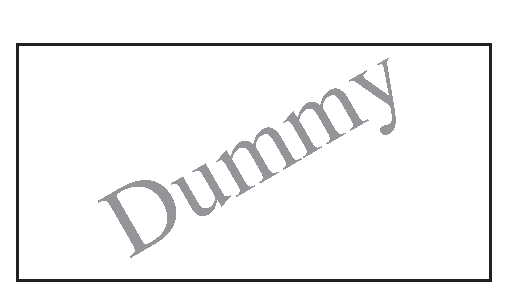
\includegraphics[width=0.5\textwidth]{img/dummy}
\caption{Utilization of four tasks on the Linux-RTXG only priority scheduling. Each tasks are given different priorities.}
\end{center}
\label{fig:rtx_prio}
\end{figure}

\begin{figure}[t]
\begin{center}
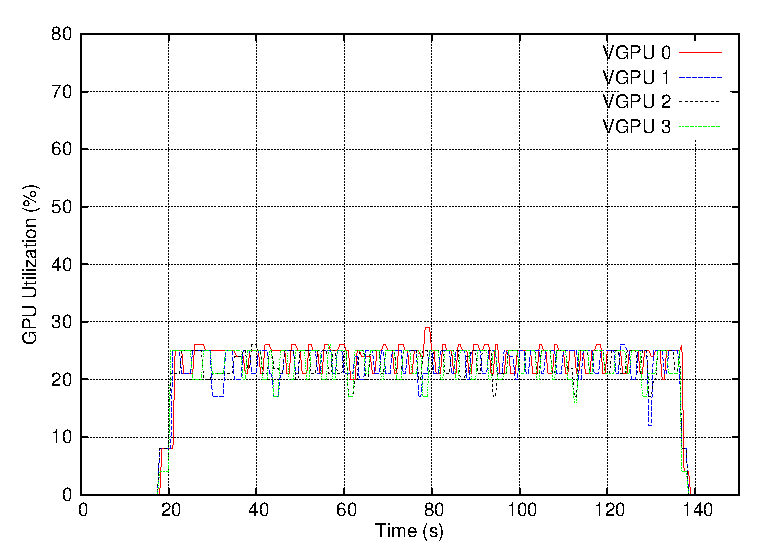
\includegraphics[width=0.5\textwidth]{img/rtx_qos.eps}
\caption{Utilization of four tasks on the Linux-RTXG resource reservation. Each tasks are given different priorities and all tasks are fairly given resources which is 25\%}
\end{center}
\label{fig:qos_rtx}
\end{figure}

\begin{figure}[t]
\begin{center}
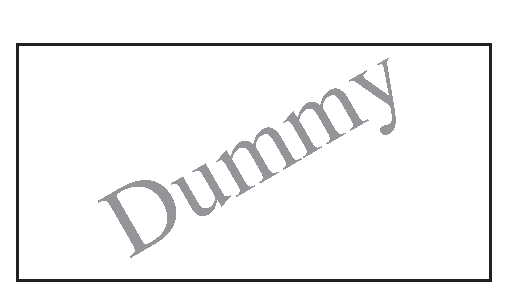
\includegraphics[width=0.5\textwidth]{img/dummy}
\caption{Utilization of four tasks on the Gdev resource resevation. All tasks are fairy given resources which is 25\%}
\end{center}
\label{fig:qos_gdev}
\end{figure}
The first, we experiment the utilization using only priority scheduling, we prepare four diffenre priorities GPU task.
As a result is showed in Figure~\ref{fig:rtx_prio}.
We can seen the the task has been used in order of priority in Figure~\ref{fig:rtx_prio}.

The second, we demonstrate performance of Linux-RTXG QoS management by using NVIDIA's proprietary software.
Maximum utilization is Minimam 


Next then, we demonstrate and compare the performance of the Linux-RTXG QoS management and the Gdev's QoS management by using Gdev's libray and Nouveau's open-source driver.
Figure~\ref{fig:qos_rtx, fig:qos_rtx} show experimental results of each tasks utlization on the Linux-RTXG QoS management and the Gdev QoS management.

A maximum utilization of Linux-RTXG is less than to x\%, while a minimum utilization of Linux-RTXG is more than to x\%.
A maximum utilization of Gdev is less than to x\%, while a minimum utilization of Gdev is more than to x\%.
Distribution of Linux-RTXG is \textbf{x}, the variance of Gdev is \textbf{x}.
We can be seen that the performance is not nearly falling from the above results
%Linux−RTXGの振幅は◯%以下であり,Nouveauの振幅は◯%以下である.
%Linux-RTXGの分散は◯であり,Nouveauの分散は◯なことから,性能はほぼ落ちていないことがわかる.
%最後に非周期タスクが存在する環境下においても,QoS Managementによってリソース制限がかかっていることを示すことで,

Therefore, the synchronization mechanism of Linux-RTXG excluding kernel modification,
it is show that possible scheduling without sacrificing performance.

%つまり,Linux-RTXGのカーネル編集を除いたシンクロナイゼーションメカニズムにおいても,
%性能を落とさずにスケジューリング可能なことを示せている.



%ここでは、今回同一アルゴリズムでQoSマネージメントを行っているGdevとの比較を行い、
%パッチを利用しない実装においても、性能をほぼ落とすこと無くできていることを示す。

%比較対象は、本Linux-RTXGと同様のスケジューリングアルゴリズムが提供可能なGdevのモジュール版とで比較する。
%評価に用いるスケジューリングポリシーはBANDスケジューラを用いる。
%実験に利用するアプリケーションとして、\ref{sec:eval:sched_overhead}節で利用したものと同様のものでTaskを4つ生成し、各タスク毎に25\%のGPU利用権限を与える。
%これらのタスクの実行中のGPU利用率を計測し、Gdevと同様のアルゴリズムを用いることで、今回提供するLinux−RTXGによるアプローチによってどれだけQoSマネージメントについてのパフォーマンスに影響するかを示す。
%Gdevを用いることから、両者ともデバイスドライバはNouveauドライバを用いる.




